\section{Introduction}

With the advent of Internet of Things, the evolution of mobile computing, and the emergence of real-time applications, the processing of an exponentially increasing volume of data must be performed in a timely fashion, i.e., with minimum latency. Despite the elasticity and vast computing power of existing cloud platforms, the access to these resources involves multiple hops of network communication, adding to the latency in which requisitions are processed. Such limitation has the following implications:

\begin{enumerate}

\item Cloud services may fail to satisfy the requirements of real-time and low-latency client applications; and

\item Offloading of delay-sensitive computation from devices with constrained resources to cloud servers (also known as Mobile Cloud Computing~\cite{}) is unlikely to work

\end{enumerate}

To reduce network latency, data processing must be performed closer to where it is produced and consumed. In accordance with this principle, the emerging paradigm of edge computing~\cite{} states that computing power should be pushed from centralized datacenters to the edge of the network. The realization of edge computing, however, still poses many challenges. 

%
First, a highly distributed edge infrastructure is not expected to exhibit virtually unlimited resources as cloud datacenters. This limitation requires an efficient usage of edge resources. Current models based on virtualization and containerization, although broadly adopted by cloud providers, may not be feasible in the context of edge computing.

Second, cloud services cover very large areas from which clients requests are always expected. In contrast, edge infrastructure features a fine-grained coverage area~\cite{5Gchallenges}, where many edge services would remain idle while in certain nodes when less clients of these services are nearby. Therefore, to optimize the usage of edge resources, service deployment to edge infrastructure should happen on-demand in an opportunistic fashion. 

%, accessible through well-known Internet names, edge services 

Finally, cloud servers should not be disregarded as a part of the Cloud-to-Edge continuum. %not sure whether to call it Cloud-to-Things or Cloud-to-Edge
. First, because client applications may still rely on Cloud backends for traditiona, non delay-sensitive computation. Second, because edge servers may be unavailable from the certain locations. Thus, client applications must rely on a runtime mechanism to discover and negotiate the use of nearby edge infrastructure. As the alternative infrastructures (including the cloud) may exhibit uneven loads in different moments, the decision of which to use, must take into account their current status as well as the client application requirements in terms of latency and computational power. 


%Finally, to avoid increasing the burden of application development, computation to be executed at the edge should follow, to the extent possible, a common architecture and implementation with respect to its cloud counterpart. The same applies to the computation that may be offloaded from resource constrained devices to nearby edge infrastructure.  

\subsection{Motivation}

\begin{figure}[htbp]
	\centering
	\subfloat[TODO: replace this image to avoid copyright problems.\label{fig:connected-vehicles}] {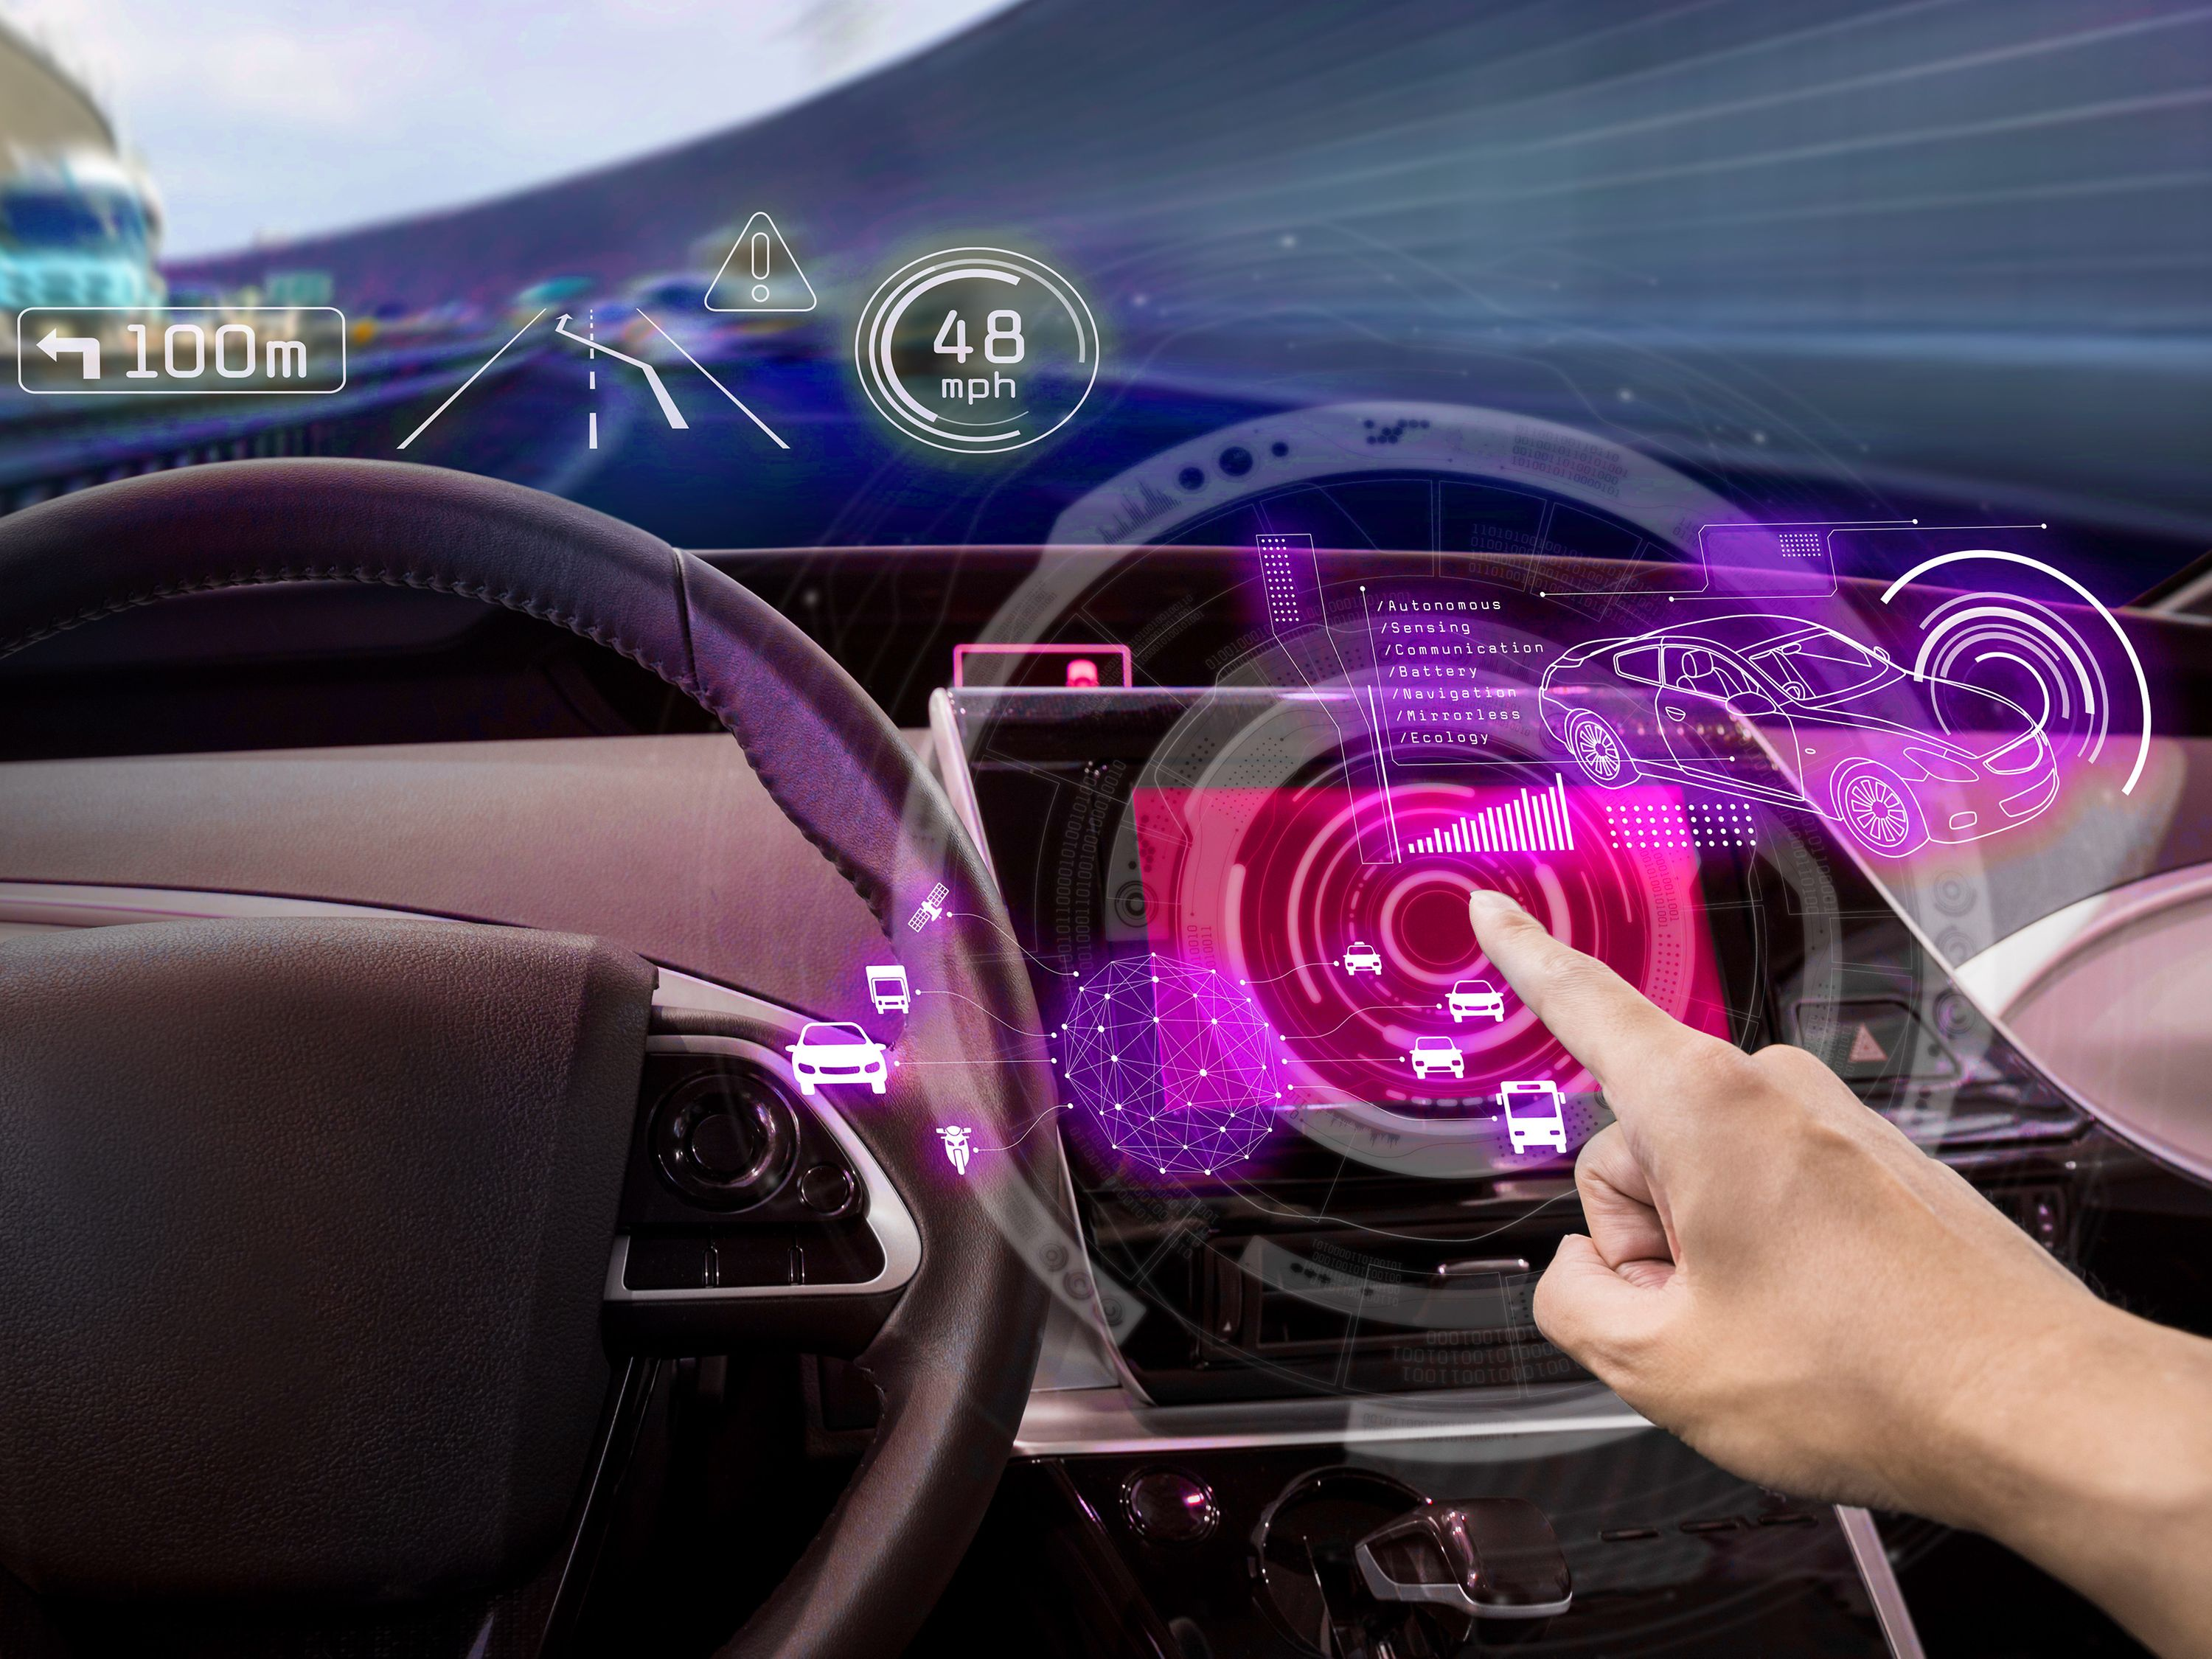
\includegraphics[width=0.47\textwidth]{figs/connected-vehicles.jpg}}\hfill
	~
	\subfloat[TODO: replace this with a less depressive image of augmented reality :)\label{fig:augmented-reality}]{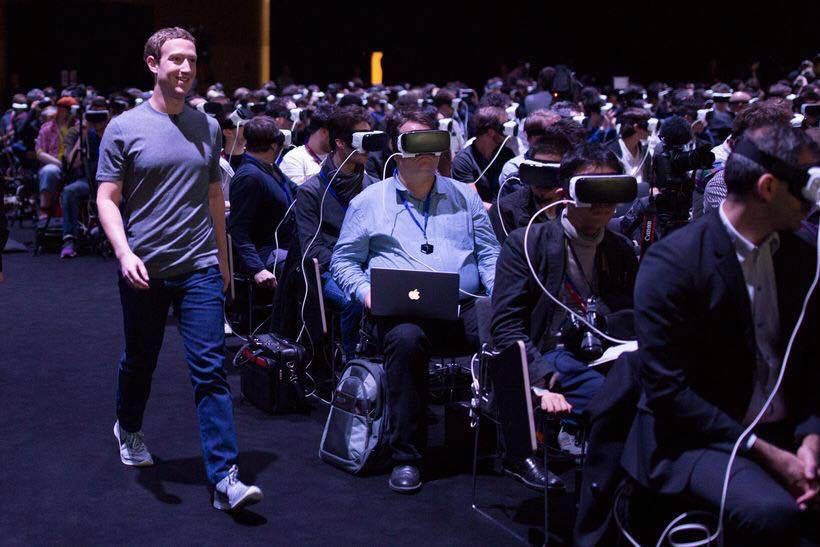
\includegraphics[width=0.53\textwidth]{figs/augmented-reality.jpg}}\hfill
	\caption{Different application types can be enabled or benefit from the low-latency of services deployed to nearby edge servers} \label{fig:motivational-cases}
\end{figure}


\subsubsection{Low-Latency Applications}

The main motivation for shifting computation from cloud to edge infrastructure is to mitigate network latency. In specific, real-time applications are the main candidates for benefiting of services deployed at nearby edge infrastructure. Among these, some have a higher degree of criticallity with respect to latency and readiness of services (e.g., delay can have severe consequences to users), whereas others can greatly benefit from lower latencies (e.g., by improving the user experience).

As an example of a critical application, connected vehicles~\cite{} are expected to be the computing device of the next decade. They are expected to generate XX petabytes of data by XXXX year~\cite{connectedCars} huge amounts of data %how much, cite survey
. In addition to the analysis performed locally, more complex data analysis shall be delegated to remote servers, which must respond quickly if the result involves critical information, e.g., the notification of an accident in the current path of the vehicle. With edge computing, computational resources located at mobile base stations or even composing the traffic infrastructure (e.g., highways) could provide low-latency services for connected vehicles passing by their coverage area.

In contrast, Augmented Reality (AR) is a type of application that would benefit from the low-latency of edge services~\cite{hu2015mobile}. These applications enrich the interaction of users with the physical
world by augmenting their vision of the reality with relevant information (e.g., historical information about buildings and monuments), modifying it (e.g., by translating captured text in a different language), or by adding virtual elements that can mimic interactions with the real world (e.g., virtual objects or creatures
from a fantasy game), or helping users fulfill physical tasks (e.g., by highlighting a free parking spot) 

AR applications commonly depend on two key computational tasks: 1) extracting features from physical elements in the captured scene; and 2) matching these features against a feature database to obtain the corresponding information to be added to the scene. 

With the advent of mobile computing, AR applications can be deployed to companion devices like smartphones, tablets, and special purpose glasses. In many cases, these applications must process large volumes of data. Plus, this data can be volatile, which further limits the feasibility of storing it locally. Instead, data must be acquired from remote services. In order to augment the reality captured live from devices camera, the AR application needs to perform its tasks in a timely fashion, which poses a strong restriction on the latency requirement for remote services consumed. As such, a cloud-based solution tends to fail to meet this requirement~\cite{ServerlessEdgeESOCC17}. 

%Additionally, image processing may over stress devices resources. This problem could be mitigated  
%architectural decision of where these tasks should be computed.

%AR applications that capture a live representation of the physical world, this reality must be augmented at real-time, meaning data must be retrieved in a timely fashion. Due to network latency, a cloud-based solution tends to fail. Accordingly, feature extraction task should be deployed near to client devices, e.g.., to edge servers. 

\begin{figure}[htbp]
	\centering
	\subfloat[first caption.\label{fig:cloud-to-edge}]{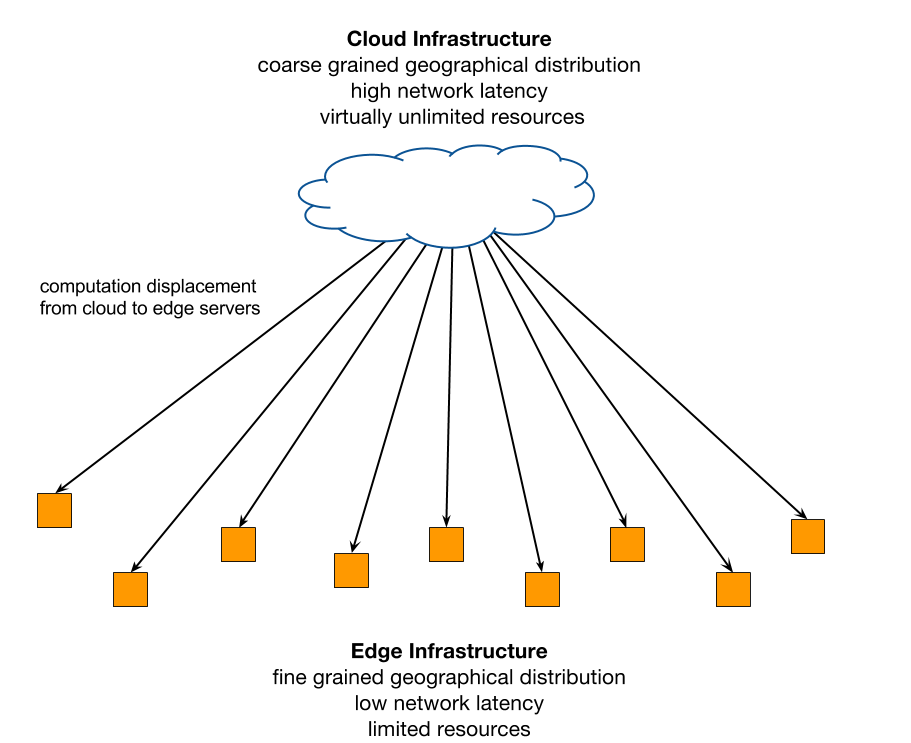
\includegraphics[width=0.49\textwidth]{figs/cloud-to-edge.png}}\hfill
	~
	\subfloat[second caption.\label{fig:mobile-to-edge}] {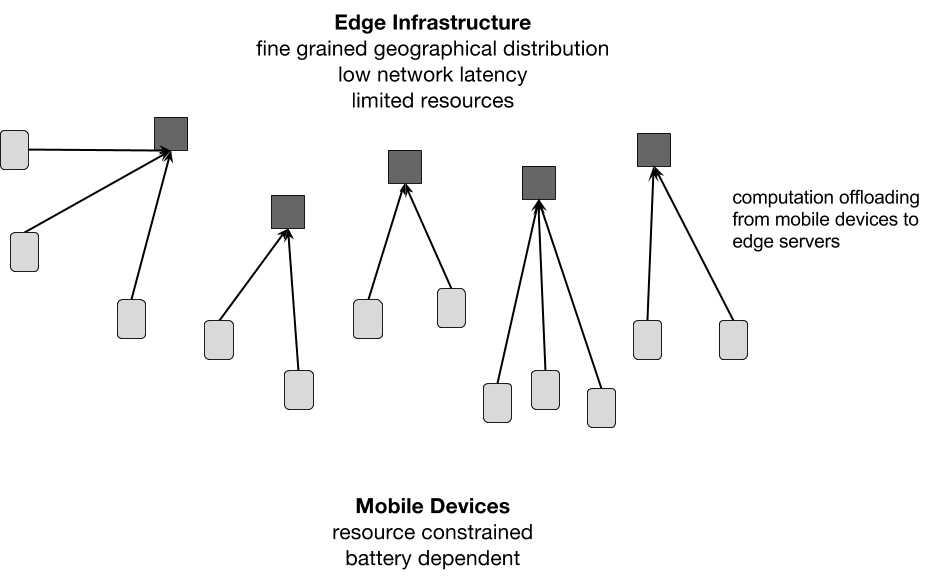
\includegraphics[width=0.49\textwidth]{figs/mobile-to-edge.png}}\hfill
	\caption{General caption.} \label{fig:1}
\end{figure}

\subsubsection{Mobile Computation Offloading}

In addition to the problem of network latency, mobile devices exhibit limitations that may further motivate the use of edge computing. 

For instance, some mobile applications rely on heavyweight tasks that can overstress the platform and limit the concurrent execution of other applications. Moreover, battery is a valuable resource that may be significantly affected by the kind of computational task performed by mobile devices. 

In the paradigm of Mobile Cloud Computing (MCC)~\cite{}, this problem has been addressed with the offloading of mobile computation to cloud servers. This approach, however, is limited by network latency. In contrast, edge computing could be an alternative to allow heavyweight or complex computation with low-latency requirements to be offloaded from resource constrained devices to nearby servers.

%The paradigm of edge computing can be explored to mitigate the problems related to the resource limitations of mobile devices. For this, heavyweight computation from mobile applications could be offloaded to nearby edge servers. 

As an example, the previously mentioned feature extraction task from MAR applications is a type of heavyweight computation based on image processing. Instead of performing it locally (as proposed in~\cite{}), mobile devices could also offload this task to nearby edge servers. 

\subsubsection{Computational Continuum}

Together, the computational resources from mobile, edge, and cloud computing have the potential of forming a \textit{\textbf{computational continuum}} on which new and disruptive types of applications can rely. 

To illustrate such scenario, we put together the two application examples previously described as part of a continuum that starts in the user's office and finishes in his home. 

In the office, let's assume the existence of a local edge server, which will be called from now on \textit{indoor-edge}. This server is owned by the company to allow employees to extend the computational capabilities of their mobile devices. Our user, e.g., makes use of an augmented reality application to TODO: describe here how an employee would use AR at work or change it to a home scenario.

Later on, the user leaves his office and enters his connected vehicle. During its way home, this autonomous vehicle will make use of nearby edge servers deployed at cellular base stations and owned by telecoms to receive low-latency updates on the best plan to reach its destination, considering the multitude of other users been driven home during the hush hour. For instance, within milliseconds, the vehicle is suggested to make a turn just in time to avoid an accident two blocks ahead. 

Already at home, the user's smartphone gets in reach of communication with the indoor edge server owned by him. In that specific day, the user found out about a new mobile game application that makes use of augmented reality. Upon installation, the edge server becomes aware of it and proceeds with the acquisition and deployment of the game components and assets that will be exposed as a service. After this, the client application, which was already running locally, becomes aware of the edge service and start consuming it with the purpose of offloading computation and preserving the smartphone resources. Not only the game performance improves, but also the battery consumption is reduced.  

In the scenario above, different types of edge infrastructure have been employed by user's devices. In specific, our idea of a computation continuum refers to the pervasiveness of computational resources and to the seamlessly transition of computation among mobile, edge, and cloud resources. Needless to say, for all the applications cited above, cloud infrastructure is  fundamental, as different services for which network latency is not disruptive are still in the cloud (e.g., authentication, persistence, large part of the business logic).



\subsection{Serverless Computing}

Serverless computing~\cite{roberts2016serverless, hendrickson2016serverless}, also known as Functions-as-a-Service (FaaS)~\cite{mateosFaas17}, emerged as an alternative execution model within cloud computing. In particular, its name derives from the fact that server management and capacity planning decisions are hidden from the software application engineers. Instead, third party providers of the serverless platform dynamically manage the allocation of machine resources for the execution of different types of computational tasks, known as \textit{functions}. Today, multiple vendors provide serverless runtime and database services. 

Among its main advantages, the serverless model is considered to be cost- and resource-efficient in comparison to virtual machine and container-based provisioning models, which generally involve significant periods of underutilization or idle time. As it has been argued elsewhere~\cite{ESOCC'17}, a serverless architecture can be employed to enable low-latency applications to make use of edge computing computational resources in an efficient and scalable way. Additionally, mobile devices could make use of compute runtimes deployed at nearby edge servers to extend their capabilities. Notwithstanding the potential of such combination, a complete model for its realization is still missing~\cite{NasticServerlessEdge17}. 

\subsection{Contributions of this Work}

In this work, we propose A3-E, a unified model for the computation continuum formed by mobile, edge, and cloud computational resources. The proposed model is strongly coped with the paradigm of serverless computing. In specific, A3-E explores the emerging execution model of FaaS to allow stateless computation to be quickly acquired, deployed, and made ready for execution. Due to the its particular characteristics, the A3-E model provides a scalable solution for the emerging paradigm of edge computing. 

As has been demonstrated with experiments, client applications can rely on dynamically and opportunistically selected services implemented as functions that are executable locally, in the edge, or in the cloud. Additionally, our experiments have shown a substantial reduction of latency when services are deployed to nearby edge infrastructure, as well as the battery consumption when computation is offloaded from mobile devices to edge servers.

%Last but not least, our contribution also includes a reference architecture for the realization of the proposed model. 

\subsection{Paper Organization}

The rest of this paper is organized as follows. Section~\ref{sec:background} provides a brief background on the main topics and concepts used by this work. Section~\ref{sec:proposal} introduces A3-E model. Section~\ref{sec:evaluation} reports on the experiments performed to evaluate our proposal with an augment reality application. Finally, Section~\ref{sec:conclusion} concludes this paper with our conclusions and future works.




